\documentclass[11pt,a4paper]{article}

% ---------------------------------------------------------------------------
% DSA4212 Team Project Report (Group 24)
% Training Small Language Models under Computational Constraints
% Figures are produced by code/plots/ in the repository.
% ---------------------------------------------------------------------------

\usepackage[utf8]{inputenc}
\usepackage[T1]{fontenc}
\usepackage{lmodern}
\usepackage[margin=2.2cm]{geometry}
\usepackage{amsmath}
\usepackage{graphicx}
\usepackage{booktabs}
\usepackage{tabularx}
\usepackage{array}
\usepackage{caption}
\usepackage{microtype}
\usepackage[hidelinks]{hyperref}
\usepackage{xurl}

\graphicspath{{figures/}}
\captionsetup{font=small,labelfont=bf,labelsep=period}
\setlength{\parskip}{0.4em}
\setlength{\parindent}{0pt}
\newcolumntype{L}{>{\raggedright\arraybackslash}X}

\begin{document}

% ---------------------------------------------------------------- title block
\begin{center}
  {\LARGE\bfseries DSA4212 Team Project Report}\\[0.4em]
  {\large Training Small Language Models under Computational Constraints}\\[1em]
  \textbf{Group 24 Members:}\\[0.2em]
  Jeon Hyewon, A0288370W\\
  Jeon Jinkyung, A0288577A\\
  Joshua Han Rui Chou, A0272122U\\
  Muhammad Umar Bin Madbi, A0272103W\\[0.6em]
  \textbf{Code and results:} \url{https://github.com/umarmadbi/dsa4212-group24-trainllm}\\[0.2em]
  {\small Every number in this report is produced from \texttt{results/} by \texttt{code/summarize.py}, each figure by a script in \texttt{code/plots/}; \texttt{docs/REPRODUCE.md} explains how to rerun any experiment.}
\end{center}

% ---------------------------------------------------------------- 1
\section{Introduction}

Language models are usually trained with thousands of GPU-hours, and most published guidance on how to spend compute comes from that scale. The Chinchilla study found that, for a fixed budget of floating-point operations (FLOPs), model size and training data should grow together, with about 20 training tokens per parameter (Hoffmann et al., 2022). In language model pretraining experiments with limited unique data and a fixed compute budget, training for up to four epochs on the same dataset yielded nearly the same loss as training on unique data (Muennighoff et al., 2023). nanoGPT and the Smol Training Playbook illustrate how engineering and data choices shape language model training under resource constraints (Karpathy, 2023; Hugging Face, 2025). Newer work proposes better optimisers, such as Muon (Jordan et al., 2024), and larger vocabularies for larger models (Tao et al., 2024).

For a small team training on a single rented GPU, the main constraint may be the time available for training. Under a time budget, a larger model learns more from every token but processes fewer tokens per second, so it reads less text in the hour; a smaller model reads more text but has less capacity to learn from it. Architectural choices, vocabulary size and optimiser overhead can all affect how many tokens the model processes within that budget. This trade-off motivates our research question. \textbf{Which training configuration gives the best performance when training a language model from scratch for one hour on a single GPU?}

Overall, our results suggest that the best use of one L4 GPU-hour is to train a larger model than Chinchilla's rule recommends (36M--65M parameters, with only 4--11 tokens per parameter), using Muon instead of AdamW, a 16,384-token vocabulary instead of 8,192, and no more than two passes over the same data. Together these changes lower test bits per byte (BPB) from 1.1994 to 1.1583 for our declared final configuration ($-0.041$), and to 1.1494 with a wider model shape ($-0.050$). Four of our seven predictions from the readings missed outright and two were only partly supported, highlighting how recommendations derived under fixed FLOP budgets may not hold under a fixed training-time budget (Section~\ref{sec:insights}).

% ---------------------------------------------------------------- 2
\section{Declared Setup}\label{sec:setup}

We documented our initial budget, initialisation and evaluation objective before training, with subsequent amendments recorded in the repository under \texttt{docs/DECLARATIONS.md}. \textbf{Compute budget.} Each training run gets 60 minutes of counted training time on one NVIDIA L4 GPU (24 GB, bf16) on Modal, long enough to pass the fastest learning phase and affordable for about 60 full runs from our pooled credit of about \$120; data loading and \texttt{torch.compile} warm-up count towards the budget, evaluation and checkpoint pauses do not, and 15-minute learning-rate pilots and tokenizer training are excluded. \textbf{Initialisation.} Every model starts from random weights (nanoGPT's GPT-2 initialisation) with our own byte-level BPE tokenizer trained on the training split, and no pretrained weights or components are used; a BPE merge table is a counting algorithm, not a neural component. \textbf{Evaluation.} We measure bits per byte (BPB) on held-out FineWeb-Edu text, using the validation split for every decision and scoring the test split once, at the end, for 57 models frozen in advance; because BPB normalises by raw UTF-8 bytes, models with different tokenizers are comparable, whereas per-token loss is not.

BPB measures how well a model predicts educational English text, rather than factual accuracy, reasoning or instruction following. We did not use downstream benchmarks such as HellaSwag: even GPT-2 (124M parameters, 10B training tokens) scores only about 30\% against 25\% for random guessing (Karpathy, 2024), and our models are smaller and trained on far less data, so such scores would provide little distinction between the configurations we compare.

Two features of a time budget shaped the design. First, \textbf{equal time is not equal compute}: larger and wider models use the GPU more efficiently, so they receive more FLOPs in the same hour. Second, \textbf{the hardware is part of the noise}: every rented L4 runs at its 72\,W power cap but at a machine-specific clock (810 to 1,058\,MHz), so identical runs can read up to 12\% different amounts of text. In five repeated runs of one configuration, 84\% of the variance in final BPB followed the number of tokens processed. Seed noise therefore had to be measured, not assumed.

% ---------------------------------------------------------------- 3
\section{Predictions Based on Prior Research}\label{sec:predictions}

We read the four starter references and followed their citations to work on optimisers, model shape and vocabulary size. Before each experiment we turned the relevant reading into a written prediction for our one-hour setting and recorded it in the decision log, so that every result could be judged against an expectation fixed in advance. Table~\ref{tab:predictions} lists the claims and our predictions; its last column summarises the outcomes reported in Section~\ref{sec:results}.

\begin{table}[ht]
\centering\small
\begin{tabularx}{\linewidth}{LLLL}
\toprule
\textbf{Reading} & \textbf{What it reports} & \textbf{Our prediction for one L4-hour} & \textbf{Outcome} \\
\midrule
Chinchilla (Hoffmann et al., 2022) & About 20 tokens per parameter for a fixed FLOP budget & Optimum 25M--35M, 10--20 tokens per parameter & Missed: 36M--65M at 4--11 tokens per parameter (Section~\ref{sec:size}) \\
Muennighoff et al.\ (2023), repetition & Up to ${\sim}4$ epochs almost as good as new data & 2 and 4 passes as good as fresh data & Missed: 4 passes already worse (Section~\ref{sec:repetition}) \\
Muennighoff et al.\ (2023), scarce data & Excess parameters lose value faster than repeats & A smaller model does better & Opposite: the largest did best (Section~\ref{sec:repetition}) \\
Smol Playbook; Allal et al.\ (2025) & Data quality and mixtures matter most & Corpora differ by about 0.01 & Partly missed: DCLM $+0.028$, mixture best (Section~\ref{sec:data}) \\
Muon (Jordan et al., 2024) & More learning per step than AdamW & Gain of 0.01--0.02 after equal tuning & Exceeded: $-0.026$ (Section~\ref{sec:muon}) \\
Kaplan et al.\ (2020); MobileLLM & Shape matters little / deep-thin best for small models & No shape clearly better & Missed: wide better through speed (Section~\ref{sec:shape}) \\
Tao et al.\ (2024) & Compute-optimal vocabulary about 5k--8k here & Best vocabulary 8k or 16k & Partly missed: 16k and 32k tie, both beat 8k (Section~\ref{sec:shape}) \\
\bottomrule
\end{tabularx}
\caption{Claims from the readings, our predictions written before each experiment, and what we found.}
\label{tab:predictions}
\end{table}

% ---------------------------------------------------------------- 4
\section{Methodology}

\subsection{Training pipeline and data}

We adapted nanoGPT, a GPT-2-style transformer (context 512 tokens, tied embeddings, no dropout) with our own 8,192-token byte-level BPE tokenizer, trained with 32,768 tokens per step, AdamW (betas 0.9, 0.95; weight decay 0.1), 200 warm-up steps and cosine decay to 10\% of the peak learning rate. We made three changes: \textbf{A clock-based schedule:} stock nanoGPT decays the learning rate over a planned number of steps, which under a time budget would leave fast models unannealed at the cap and cut slow ones off mid-decay; our cosine decay follows the fraction of the 3,600 counted seconds used, so every run finishes annealing exactly at 60 minutes. \textbf{Checkpoint and resume} that carries the counted time, random states and data position, so a preempted run continues without resetting its budget. \textbf{A deterministic BPB evaluator} and a 13-gram contamination check between evaluation and training documents.

We used FineWeb-Edu (sample-10BT) as our main training corpus because it matches our focus on educational English text, performed well in small-scale comparisons, and provides more data than a model can process in one hour (Penedo et al., 2024). In the data experiment, we compared it with FineWeb to assess the effect of the educational filter and with DCLM-baseline as an alternative corpus selected by a different classifier (Li et al., 2024). English Wikipedia is used only for evaluation. Corpora were split by document before tokenizer training (about 10\,MB each for validation and test, duplicates removed), and each has 2.45 to 2.57 billion training tokens, at least 1.5 times what the fastest model reads in an hour, so outside the repetition experiment no run sees text twice.

\subsection{Experimental protocol}\label{sec:protocol}

\textbf{One change at a time.} We first chose the model size by experiment, then changed one factor at a time from that baseline (data, repetition, optimiser, shape, vocabulary) and finally combined the changes that helped. The baseline, N49 (11 layers of width 576, 48.8M parameters), was selected by a rule fixed before the size results were known.

\textbf{Equal tuning effort.} Because a method compared against a poorly tuned baseline looks better than it is, every configuration received the same learning-rate protocol: four peak rates a factor of 2 apart in 15-minute pilots, one more rate if the best was at the edge of the grid, three seeds for any close call, and a 60-minute check that the 15-minute choice still wins over the full hour. Across all sizes the best rate was $2\times10^{-3}$ or $4\times10^{-3}$, within noise of each other.

\textbf{Decision rules fixed before results.} The pooled seed-to-seed standard deviation of 60-minute runs is 0.0057 BPB. A difference counts as real only if it exceeds two standard errors: 0.0132 for one run against a 3-seed mean and 0.0091 for three seeds against three; smaller differences are reported as inconclusive. Comparisons on the four-set average (AVG4, Section~\ref{sec:data}) use that average's own seed spread (0.0055), giving a three-seed threshold of 0.0088. Each experiment's question, prediction, decision rule and follow-up triggers were written into the decision log (\texttt{docs/decisions.md}, D01 to D47) before its first run. The test set is locked in code: the scoring script refuses any model not listed in \texttt{configs/frozen\_configs.yaml}, which was committed before any test score existed. In total the project used 270 Modal jobs (59 complete 60-minute runs and 118 shorter pilots), about 98 L4-hours and about \$79 of credit.

% ---------------------------------------------------------------- 5
\section{Experiments and Results}\label{sec:results}

\subsection{Model Size and Training Efficiency}\label{sec:size}

Applying Chinchilla's rule to the compute an L4 delivers in an hour, we predicted an optimum of 25M to 35M parameters. Seven sizes from 7M to 65M were each trained for exactly 60 minutes at their own tuned learning rate (Figure~\ref{fig:size}).

\begin{figure}[ht]
\centering
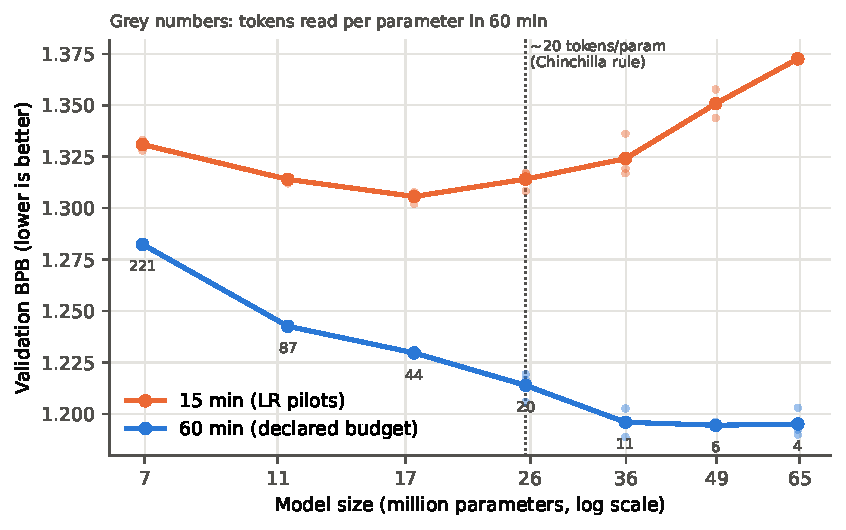
\includegraphics[width=0.62\linewidth]{size_vs_bpb.pdf}
\caption{Validation BPB against model size after 15 minutes (orange) and 60 minutes (blue); faint dots are seeds and grey numbers give tokens read per parameter in 60 minutes. The dotted line marks the 26M model, which reads Chinchilla's ${\sim}20$ tokens per parameter.}
\label{fig:size}
\end{figure}

At 60 minutes the loss falls until 36M parameters and then flattens. The 36M, 49M and 65M models agree within 0.0015 BPB (threshold 0.0091) despite processing only 4--11 tokens per parameter, while the 26M model, which reads Chinchilla's 20 tokens per parameter, is worse by 0.018 (about three standard deviations). Performance is flat above the optimum but worsens sharply below it. Increasing the size to 65M raises BPB by only 0.0006 relative to the best model, while reducing it to 7M raises BPB by 0.088. As training time increases from 15 to 60 minutes, the optimal size shifts from around 17M to 50M--70M parameters, growing roughly in proportion to the time budget rather than following Chinchilla's square-root relationship.

\textbf{Why the prediction missed.} We had expected the lower GPU efficiency of small models to pull the optimum smaller, but the effect runs the other way. Larger models use the L4 better (model FLOPs utilisation 0.18 at 7M against 0.24 at 65M), allowing more computation per hour. However, this was not the main reason for the difference. Fitting a Chinchilla-style law,
\begin{equation}
  L(N, D) = E + \frac{A}{N^{a}} + \frac{B}{D^{b}},
  \label{eq:law}
\end{equation}
to our 14 complete runs (largest residual 0.013 BPB), where $N$ is the number of parameters, $D$ the number of training tokens and $E$, $A$, $B$ fitted constants, gives $a = 0.16$ and $b = 0.84$. This suggests an equal-FLOP optimum of approximately 56M parameters (leave-one-out range 40--60M) and 4.8 tokens per parameter, compared with 27M parameters and 20 tokens per parameter under Chinchilla's published law. In our setting, loss falls quickly with additional data and slowly with parameters, making extra model capacity more valuable after a few hundred million tokens. We also saw a winner's curse: the first seed of both the 36M and 65M models ran on fast machines and was each size's best result, and only three seeds revealed the tie. By the pre-declared rule, N49 became the baseline for all later experiments.

\subsection{Data Quality and Generalisation}\label{sec:data}

Since a model always scores best on text like its training data, we declared in advance that corpora would be judged on the average over four validation sets (AVG4), including Wikipedia, which no model trains on, and predicted differences of about 0.01 BPB.

\begin{table}[ht]
\centering\small
\begin{tabular}{lccccc}
\toprule
\textbf{Trained on (N49, 3 seeds)} & \textbf{FineWeb-Edu} & \textbf{FineWeb} & \textbf{DCLM} & \textbf{Wikipedia} & \textbf{AVG4} \\
\midrule
FineWeb-Edu & 1.1945 & 1.3850 & 1.5404 & 1.4616 & 1.3954 \\
FineWeb (unfiltered) & 1.2680 & 1.3324 & 1.5128 & 1.4744 & 1.3969 \\
DCLM & 1.2763 & 1.3819 & 1.3622 & 1.4490 & 1.3673 \\
60/40 FineWeb-Edu + DCLM & 1.2167 & 1.3713 & 1.3811 & 1.4150 & 1.3460 \\
\bottomrule
\end{tabular}
\caption{Validation BPB on four held-out sets for the same model trained for one hour on each corpus. AVG4 differences above 0.0088 are real (Section~\ref{sec:protocol}).}
\label{tab:data}
\end{table}

Data filtering improves performance on its target domain, while combining datasets leads to better generalisation. FineWeb-Edu's educational filter gains 0.07 to 0.08 BPB on educational text, but this advantage does not carry over to other text. Its AVG4 (1.3954) is essentially the same as that of unfiltered FineWeb (1.3969). DCLM, which uses a different quality classifier, achieves an AVG4 lower than FineWeb-Edu's by 0.028 (about five standard deviations) and is the best of the three single corpora on Wikipedia. Since each filtered corpus won clearly on some text, a pre-declared follow-up ran a 60/40 mixture of FineWeb-Edu and DCLM, which beats DCLM on AVG4 by 0.021 and on Wikipedia text by 0.034, at a cost of 0.022 on FineWeb-Edu. These findings remained consistent after removing 145 near-duplicate validation documents, adjusting for machine speed and re-checking each corpus's learning rate. A small model trained for one hour has limited capacity, so the best training corpus depends on the target text, as specialising in one domain may reduce performance elsewhere. AVG4 was declared as the criterion for this data comparison only. Before any data run, we declared that later experiments would train on FineWeb-Edu regardless of the result, since our objective is FineWeb-Edu BPB (Section~\ref{sec:setup}). The mixture is our recommendation when the target is broad text.

\subsection{Effects of Data Repetition}\label{sec:repetition}

We gave N49 its usual hour on a random subset of FineWeb-Edu sized so that the hour reads it about 2, 4, 8, 16 or 32 times. Following Muennighoff et al.\ (2023), we predicted that 2 and 4 passes would be indistinguishable from fresh data.

\begin{figure}[ht]
\centering
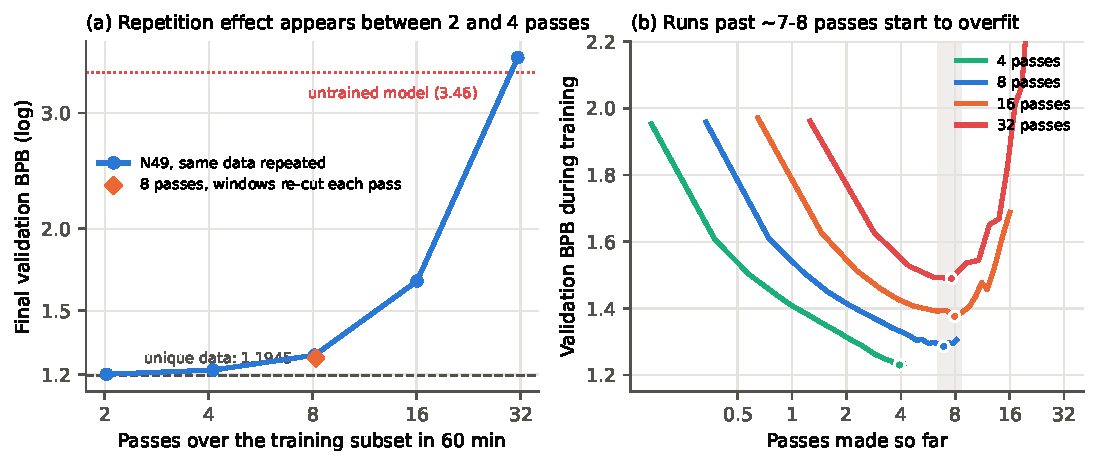
\includegraphics[width=\linewidth]{repetition.pdf}
\caption{(a) Final validation BPB against passes over the training subset (3 seeds at 2, 4 and 8 passes); dashed: unique data, dotted: untrained model, diamond: windows re-cut every pass. (b) Validation BPB during training against passes made so far; dots mark each run's minimum.}
\label{fig:repetition}
\end{figure}

The effects of data repetition appeared earlier than expected (Figure~\ref{fig:repetition}a). Two passes increased BPB by 0.0066 (3 seeds, below the 0.0091 threshold), four passes $+0.024$ and eight passes $+0.090$; at 32 passes the model ends worse on unseen text (3.64 BPB) than an untrained model (3.46), suggesting that it had memorised its 9-million-token training subset. As shown in Figure~\ref{fig:repetition}b, validation BPB reaches its minimum after approximately 7--8 passes in the longer runs before increasing, indicating overfitting as training continues. Using the loss law fitted in Section~\ref{sec:size}, we converted each run's BPB into the amount of fresh data that would give the same loss. A second pass was worth 74--98\% of fresh data across seeds, and at eight passes the text read was worth only 35--42\%. Beyond eight passes, effective data decreases, a pattern not captured by the saturating formula of Muennighoff et al.

We conducted two pre-declared follow-up experiments. \textbf{First, does model size affect overfitting?} Following the paper, we expected smaller models to do better on the same 36M-token subset. However, the 65M model performed best (1.2688 BPB against 1.2933 for N49) and the 17M model worst (1.3036). Under a time budget, larger models process fewer tokens and therefore repeat the data less often. The 65M model completed only 6.6 passes in the hour, while the 17M model read it 22 times, exceeding the point where overfitting began. \textbf{Second, does repeating identical samples affect performance?} Our loader repeated exactly the same 513-token windows every pass. Changing the window boundaries between passes cut seed 0's eight-pass penalty from 0.099 to 0.077. However, both findings are based on single runs and should be interpreted cautiously. The remaining differences from the paper may also be due to our training settings, which were optimised for unique data and did not include dropout.

\subsection{Optimiser Performance: Muon vs AdamW}\label{sec:muon}

Unlike AdamW, which updates weights individually, Muon updates entire weight matrices by orthogonalising their momentum using five Newton--Schulz iterations (Jordan et al., 2024). These extra multiplications cost time, which is our budget. We applied PyTorch's Muon to the 44 hidden matrices (43.8M of N49's 48.8M parameters), kept AdamW for embeddings and LayerNorms, scaled Muon's update to AdamW's size (Liu et al., 2025), and gave Muon exactly the tuning protocol AdamW received. We predicted a BPB gain of 0.01--0.02.

\begin{figure}[ht]
\centering
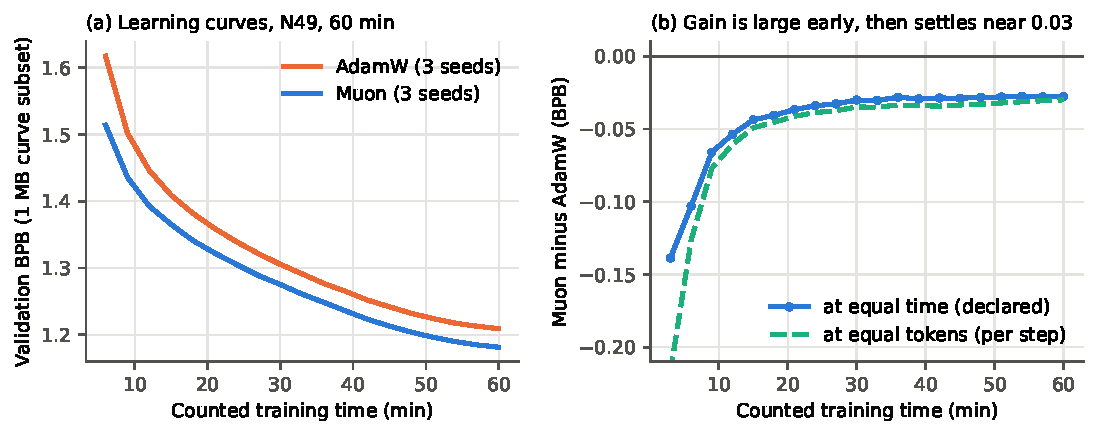
\includegraphics[width=0.95\linewidth]{muon_curves.pdf}
\caption{(a) Mean learning curves of AdamW and Muon at N49 (3 seeds each). (b) Muon minus AdamW along the hour, at equal training time (solid) and at an equal number of tokens processed (dashed).}
\label{fig:muon}
\end{figure}

Muon achieved a BPB of 1.1683 compared with AdamW's 1.1945, an improvement of 0.026 across three seeds each. It also outperformed AdamW on all four validation sets and the test set. As shown in Figure~\ref{fig:muon}b, the improvement was greatest early in training ($-0.14$ after 3 minutes) before settling near $-0.03$ in the second half hour ($-0.026$ at the end on the full validation set), suggesting that Muon mainly improves learning efficiency. The equal-token curve lies only about 0.002 below the equal-time curve, indicating that Newton--Schulz's 3--5\% throughput overhead had little impact on performance. Muon's best learning rate matched AdamW's ($2\times10^{-3}$), supporting the effectiveness of update-size matching. Muon also showed greater consistency across seeds, with a fivefold smaller spread (0.0003 versus 0.0014).

\subsection{Effects of Model Architecture and Vocabulary Size}\label{sec:shape}

At approximately 49M parameters, we compared the baseline ($11 \times 576$) with shallow-wide ($6 \times 768$) and deep-narrow ($19 \times 448$) architectures. Given the contrasting findings of Kaplan et al.\ (2020) and MobileLLM (Liu et al., 2024), we predicted no clear winner. We also tested vocabulary sizes of 4,096, 16,384 and 32,768 tokens while keeping the transformer blocks fixed (43.8M non-embedding parameters). Based on Tao et al.\ (2024), which suggests an optimal vocabulary of 5k--8k for our compute budget, we predicted that 8k or 16k would perform best (Table~\ref{tab:shape}).

\begin{table}[ht]
\centering\small
\begin{tabularx}{\linewidth}{>{\raggedright\arraybackslash}p{3.5cm} >{\centering\arraybackslash}p{1.0cm} >{\centering\arraybackslash}p{1.7cm} >{\centering\arraybackslash}p{1.8cm} >{\centering\arraybackslash}p{1.8cm} L}
\toprule
\textbf{Change from baseline} & \textbf{Seeds} & \textbf{Tokens/s vs baseline} & \textbf{Validation BPB} & \textbf{Difference} & \textbf{Diagnostic} \\
\midrule
Baseline: $11\times576$, 8k vocabulary & 3 & -- & 1.1945 & -- & -- \\
Shape $6\times768$ (wide) & 1 & $+15.8\%$ & 1.1768 & $-0.018$ & Tie at equal steps ($-0.002$) \\
Shape $19\times448$ (deep) & 1 & $-12.4\%$ & 1.2158 & $+0.021$ & Worse at equal steps ($+0.015$) \\
Vocabulary 4,096 & 1 & $+2.5\%$ & 1.2032 & $+0.009$ & Close call, not resolved \\
Vocabulary 16,384 & 3 & $-10.5\%$ & 1.1781 & $-0.016$ & $-0.013$ with overlapping windows \\
Vocabulary 32,768 & 1 & $-25.0\%$ & 1.1774 & $-0.017$ & $-0.011$ with overlapping windows \\
\bottomrule
\end{tabularx}
\caption{Shape and vocabulary experiments at about 49M parameters. Single-seed verdicts use the 0.0132 threshold.}
\label{tab:shape}
\end{table}

\textbf{Shape.} The wide model wins only because its larger matrix multiplications run faster on the L4 (utilisation 0.26 against 0.22), so it reads 16\% more text; at an equal number of steps it ties with the baseline. The deep model runs more, smaller operations in sequence and loses both per step and in speed. Under a time budget an architecture is partly judged by how efficiently the hardware runs it, so this result is specific to the L4.

\textbf{Vocabulary.} Both 16k and 32k beat 8k by about 0.016 and tie with each other. The 32k model processes 25\% fewer tokens per second, but each token holds more text, so it reads only 11\% less text in the hour and still wins. We then found a confound in our own measurement: scoring uses non-overlapping 512-token windows, and at a larger vocabulary 512 tokens hold more text (1.75\,kB at 4k against 2.34\,kB at 32k), so predictions see more context even if the model is no better. Re-scoring every model with overlapping windows, which gives each token at least 384 tokens of context, shrinks the gaps by about 0.003 at 16k and 0.006 at 32k without changing the order, so most of the gain (about four fifths at 16k, two thirds at 32k) reflects a better model of the text.

\subsection{Combined Improvements and Test Results}\label{sec:combined}

We expected the three improvements to have diminishing combined benefits, as Muon and the 16k vocabulary increase training time per step, potentially reducing the wider model's speed advantage. We therefore tested two configurations, each with separately tuned learning rates and three seeds: recipe B (RB: Muon and 16k vocabulary with the baseline architecture) and recipe A (RA: Muon, 16k vocabulary and the wider $6 \times 768$ architecture). RB was pre-declared as the final configuration unless RA exceeded the performance threshold, since RB required fewer changes and was less dependent on L4-specific hardware efficiency.

\begin{figure}[ht]
\centering
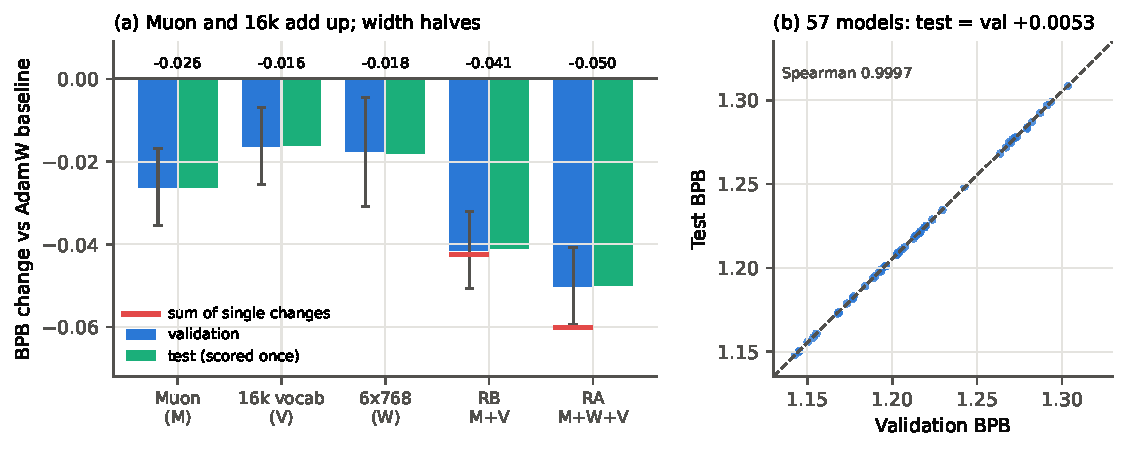
\includegraphics[width=\linewidth]{recipe_and_test.pdf}
\caption{(a) BPB change against the AdamW baseline for each change alone and for the two recipes, on validation (blue, 2-SE bars) and test (green); red marks: sum of the single changes. (b) Validation against test BPB for the 57 frozen models (two heavy-repetition models lie off the axes).}
\label{fig:recipe}
\end{figure}

Figure~\ref{fig:recipe}(a) shows which gains combine. Muon and the 16k vocabulary add almost exactly: RB improves by 0.041 against a sum of 0.043. Width does not: inside the recipe it adds 0.009, half of its 0.018 alone, even though RA still ran about 17\% faster than RB (1\% more tokens per second than the baseline, against 14\% fewer for RB). This suggests that additional tokens provide diminishing benefits when the optimiser already improves learning efficiency. RA outperforms RB by 0.0087, just 0.0004 below our pre-declared threshold. RB therefore remains our final configuration, while RA achieves the best measured performance. Using the smaller seed variation observed in these configurations, the difference would be statistically significant (two standard errors $= 0.0034$). On the test set, RB scores $1.1583 \pm 0.0025$ and RA $1.1494 \pm 0.0011$ against the baseline's $1.1994 \pm 0.0015$, improvements of 0.041 and 0.050. Removing contaminated documents or using overlapping evaluation windows changes these improvements by at most 0.003 BPB. To check whether repeated decisions based on validation results led to overfitting, Figure~\ref{fig:recipe}b compares validation and test BPB across all 57 frozen models. Test BPB is consistently about 0.0053 higher than validation BPB, with a Spearman rank correlation of 0.9997. This strong agreement suggests that the improvements observed during validation also generalise to the held-out test set.

% ---------------------------------------------------------------- 6
\section{Experimental Challenges and Key Insights}\label{sec:insights}

Four of our seven predictions missed outright and two were only partly right (Table~\ref{tab:predictions}), for three reasons. First, a time budget prices choices by speed on real hardware, not by FLOPs. The wide shape won only through speed, and larger models overfitted less because they read limited data fewer times. Second, published laws may not hold at our much smaller scale and with our settings, which explains the size and repetition misses. Third, the measurement can move with the quantity measured: part of the vocabulary gain came from longer evaluation contexts.

We also logged process failures that would have silently biased a time-budget comparison, including two pilots that skipped the counted compile warm-up by reusing a warm container, a resume bug that appeared only on the GPU, a summary script that did not apply the declared ranking rule, and a fit with its equations in the wrong order (it placed the optimum at 20.7M). Each was fixed and logged, and every figure and table in this report is now checked against the raw results.

% ---------------------------------------------------------------- 7
\section{Discussion}

For a team with one GPU-hour, our results suggest training a model larger than Chinchilla's rule recommends (about 5 rather than 20 tokens per parameter), using Muon, preferring a 16k vocabulary over 8k at 50M parameters, choosing the shape that runs fastest on the available GPU, choosing the corpus by the target text, and avoiding more than two passes over the same data. Beyond these configurations, the experiments point to four broader lessons.

\textbf{Short comparisons can overstate an improvement.} Muon's advantage was $-0.059$ BPB after 15 minutes but $-0.026$ after 60, because most of its gain comes early in training ($-0.14$ at 3 minutes). Judged on our 15-minute pilots, Muon would have looked more than twice as good as it is. A new optimiser therefore has to be compared at the full budget and with equal tuning, which is how we obtained a smaller but more reliable gain. Muon's seed-to-seed spread was also five times smaller than AdamW's.

\textbf{Gains combine only when they act through different routes.} Muon and the 16k vocabulary added almost exactly (0.041 combined against 0.043 summed), but the wider shape kept only half of its 0.018 standalone gain once Muon was in place. Width helps by reading more text in the hour, and extra text is worth less when the optimiser already learns more from each token. A practitioner can use this to predict which changes are worth combining before running them.

\textbf{A fixed time budget changes the advice for limited data.} Muennighoff et al.\ recommend a smaller model when unique data is scarce. Under a time budget we found the opposite: on the same 36M-token subset, the 65M model did best because it read the data only 6.6 times, while the 17M model passed the point where overfitting began. When data is limited and time is fixed, enlarging the model is a better use of the hour than adding passes. More generally, the optimum on model size was asymmetric: the 65M model was only 0.0006 BPB worse than the best size, but the 7M model was 0.088 worse, so a team unsure of the optimum should err towards a larger model. The best size also grew roughly in proportion to training time between 15 and 60 minutes. If this trend continues, a longer budget would favour a proportionally larger model, although our two horizons cannot confirm it.

\textbf{Under a time budget, the hardware and the evaluation are part of the result.} 84\% of the seed-to-seed variance in our repeated runs came from differences in machine speed, the wide shape won only because the L4 runs its larger matrix multiplications faster, and part of the vocabulary gain came from longer evaluation contexts rather than a better model. Before crediting a modelling change, it is worth checking whether it changed throughput or the measurement instead.

\textbf{Limitations.} All runs used one GPU type, so speed-driven results (shape, vocabulary cost) may not transfer, and after Section~\ref{sec:size} every factor was tested at 49M parameters only. The one-hour budget excludes learning-rate pilots and tokenizer training, as the brief allows, so our results describe training efficiency per run rather than the full cost of finding a good configuration: the final 60-minute runs used about 59 of the project's 98 L4-hours. Several verdicts rest on one seed by the declared rule; the fitted scaling law is loosely determined (leave-one-out optimum 40--60M); the best vocabulary sits at the top of the tested grid; context length and batch size were not tested; and Muon's own hyperparameters were left at their defaults. The repetition results may depend on the fixed training windows and the absence of dropout, and BPB measures prediction of educational text, not downstream ability (Section~\ref{sec:setup}).

\textbf{Future work.} Repeating the size and shape comparisons on a second GPU type would separate hardware effects from modelling effects; a third horizon (for example two hours) would test whether the optimal size keeps growing with time; and extending the vocabulary to 65k and adding regularisation under repeated data would answer the two most direct open questions.

% ---------------------------------------------------------------- 8
\section{Conclusion}

Most published results we tested did not transfer unchanged to a one-hour budget, because a time budget prices every choice by its throughput on real hardware rather than by its FLOPs. Our final recipe improves test BPB by 0.041 over a tuned AdamW baseline, and every decision was reached under rules fixed in advance and confirmed once on a locked test set.

% ---------------------------------------------------------------- references
\section*{References}
{\small\raggedright
\begin{list}{}{\leftmargin=1.5em \itemindent=-1.5em \itemsep=0.15em \parsep=0pt}
\item Allal, L. B., et al. (2025). SmolLM2: When smol goes big. Data-centric training of a small language model. arXiv:2502.02737.
\item Hoffmann, J., et al. (2022). Training compute-optimal large language models. \emph{Advances in Neural Information Processing Systems 35}. arXiv:2203.15556.
\item Hugging Face (2025). The Smol Training Playbook: The secrets to building world-class LLMs. \url{https://huggingface.co/spaces/HuggingFaceTB/smol-training-playbook}
\item Jordan, K., et al. (2024). Muon: An optimizer for hidden layers in neural networks. \url{https://kellerjordan.github.io/posts/muon/}
\item Kaplan, J., et al. (2020). Scaling laws for neural language models. arXiv:2001.08361.
\item Karpathy, A. (2023). nanoGPT. \url{https://github.com/karpathy/nanoGPT}
\item Karpathy, A. (2024). Reproducing GPT-2 (124M) in llm.c in 90 minutes for \$20. \url{https://github.com/karpathy/llm.c/discussions/481}
\item Li, J., et al. (2024). DataComp-LM: In search of the next generation of training sets for language models. arXiv:2406.11794.
\item Liu, J., et al. (2025). Muon is scalable for LLM training. arXiv:2502.16982.
\item Liu, Z., et al. (2024). MobileLLM: Optimizing sub-billion parameter language models for on-device use cases. \emph{ICML 2024}. arXiv:2402.14905.
\item Muennighoff, N., et al. (2023). Scaling data-constrained language models. \emph{Advances in Neural Information Processing Systems 36}. arXiv:2305.16264.
\item Penedo, G., et al. (2024). The FineWeb datasets: Decanting the web for the finest text data at scale. arXiv:2406.17557.
\item Tao, C., et al. (2024). Scaling laws with vocabulary: Larger models deserve larger vocabularies. arXiv:2407.13623.
\end{list}
}

% ---------------------------------------------------------------- AI use
\section*{Use of AI Tools}

We used AI assistants (mainly Claude by Anthropic) throughout the project: to generate and discuss ideas, to write and debug code, and to draft and edit this report. We also used them to help with decisions while building the models, for example when weighing which experiment to run next, which gaps to check before a run and how to set decision rules. Every decision was discussed and made by the team, all code was run and tested by us, and every number in this report was checked against the result files in the repository; several errors in analysis code, including those described in Section~\ref{sec:insights}, were found through these checks.

\end{document}
